\section{FLP Impossibility Theorem}

The domain of distributed systems say a major breakthrough in 1978 when Leslie Lamport in his paper "\href{https://amturing.acm.org/p558-lamport.pdf}{Time, Clocks, and the Ordering of Events in a Distributed System}" introduced the concept of logical clocks. Effectively, this paper presented an affirmative answer to the following question:

\begin{quotebox}{1978 Leslie Lamport}
    Can we impose total ordering to events received by different nodes in a distributed system?
\end{quotebox}

As a primer, a partial ordering is an order on a set of elements which satisfies the following properties:
\begin{itemize}
    \item \textbf{Reflexivity}: $a \leq a$ i.e an element is always ordered with itself
    \item \textbf{Antisymentry}: If $a \leq b$ and $b \leq a$, then $a = b$, i.e. no two distinct elemts precede each other.
    \item \textbf{Transitivity}: If $a \leq b$ and $b \leq c$, then $a \leq c$, i.e. if $a$ precedes $b$ and $b$ precedes $c$, then $a$ precedes $c$.
\end{itemize}

A total ordering is a partial ordering which satisfies the following additional property that each pair of elements is comparable, i.e. for any two elements $a$ and $b$, either $a \leq b$ or $b \leq a$.

This seemed at the time to be promising for the distributed systems community, as it lead to seeming guarantees of consensus over a strict order in distributed systems. 

However, a paper that came out in 1985 by Fischer, Lynch and Paterson, titled "\href{https://groups.csail.mit.edu/tds/papers/Lynch/jacm85.pdf}{Impossibility of Distributed Consensus with One Faulty Process}" showed the following claim is not always true: 

\begin{quotebox}{1985 Fischer, Lynch, Paterson}
    Can we always come up with a way of getting computers to agree on a common value in a distributed system, even if some of the computers are faulty?
\end{quotebox}

This paper is often referred to as the \textbf{FLP Impossibility Theorem}. Let's understand this further.

\subsection{The FLP Impossibility Claim}

We take the FLP paper's abstract verbatim that reads the following:

\begin{quotebox}{FLP Impossibility Theorem abstract}
    The consensus problem involves an \textbf{asynchronous system} of \textbf{processes}, some of which may be \textbf{unreliable}. The problem is for the \textbf{reliable processes to agree} on a binary value. In this paper, it is shown that every protocol for this problem has \textbf{the possibility of nontermination}, even with only \textbf{one faulty process}. 
\end{quotebox}

The key takeaway from this abstract, without key terms being defined is: If we exist in a distributed system where each "process" / node is willing to participate in a consensus protocol, which may take infinite amount of time to reach a consensus, with message delays being unbounded, with at-most one process being faulty, i.e. dies without notice to others, then it is not always possible to reach to a common global value.

Before we establish this however, we need to define some key concepts:

\subsection{Key concepts}

\begin{wrapfigure}{r}{0.30\textwidth}
    \centering
    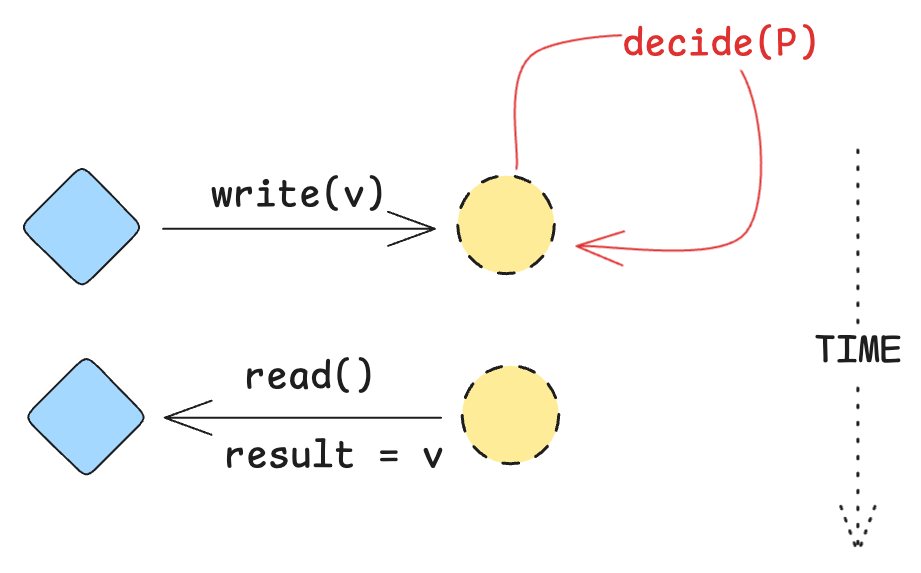
\includegraphics[width=0.30\textwidth]{general-problems/assets/flp-single-node-read-write.png}
    \caption{The single node case of read and write}
    \label{fig:flp-single-node-read-write}
\end{wrapfigure}

Let's begin with a setting which is not distributed in nature. Consider a client process $\verb|CL|$ and a server node $S$. The server $S$ saves a single bit value with itself and presents two distinct operations to the client $\verb|CL|$: 
\begin{itemize}
    \item \code{write(v: 0/1)}: This operation writes the value of a variable given by client at the server $S$.
    \item \code{read() $\to$ 0/1}: This operation returns the value of a variable stored at the server $S$.
\end{itemize}

A crucial component in this system is existence of a function $\verb|decide()|$, which can be anything that operates on the internal state of the server. A simplest form of $\verb|decide()|$ could be a function that returns the latest value stored in the server. Another variant could be a function that returns the XOR value of the last $5$ writes.

In our case, we can extend the same construction but to a distributed system outwardly presenting itself as a unit but internally being composed of multiple servers called \textbf{node}s. In essence, we desire that the same $\verb|write()|$, $\verb|read()|$ and $\verb|decide()|$ functions that were present in the single node case, be present in the distributed system as well and \textbf{they should act exactly the same}.

The FLP paper imagines the distributed setting to be describable as follows:

There are $n$ nodes in the distributed system. The nodes are connected to each other in connected but not necessarily a complete way in a graph-theoretic sense (a.k.a between any two nodes a path exist but not necessarily of length 1). Each process $p_i$ is defined by $p_i = (I_i, O_i, f_i)$ where $I_i$ is input in the set $\{0, 1\}$, $O_i$ is a one-time write only output in the set $\{\phi, 0, 1\}$, $\phi$ being the value it exercise if it has not yet been written to, and $f_i$ is a deterministic function that defines the internal state transition algorithm of $p_i$.

Each process $p_i$ can send a message $m \in M$ ($M$ being the "message universe") to some other process $p_x$ at any time as a tuple $(p_x, m)$ submitted to a globally singleton multi-set \textbf{message buffer} (note, source $p_i$ is not described in the tuple).

The \textbf{message buffer} is a special non-deterministic (the only component in the system that is not deterministic) entity that presents each process with a function \code{receive(i) $\to$ $\{\phi, m\}$}. This function when called with index $i$, either returns $\phi$, a null message or $m$, one of the messages the buffer has received for delivery to process $p_i$. In the latter case, upon delivering the message, a tuple $(p_i, m)$ is removed from the message buffer. Note how message buffer sufficiently describes an asynchronous message passing system. It can choose to returen the null message any number of times, in effect simulating unbounded delay.

In a \textbf{synchronous} setting however, we have some upper bound on the time it takes for a message to be delivered. In an \textbf{asynchronous} setting, we have no such bound. As such, it is impossible to detect if the counterparty process has failed or is just taking a long time to respond.

One should also discuss a bit about what it means to "fail" in a distributed system. Typically we categorize failures in 4 different categories:
\begin{itemize}
    \item \textbf{Fail-stop}: The process halts, notifies everyone of its death and does not respond to any further messages.
    \item \textbf{Crash}: The process halts, does not notify anyone of its death and does not respond to any further messages.
    \item \textbf{Byzantine}: The process can send arbitrary messages to other processes, including lying about its own state.
    \item \textbf{Permissionless Byzantine}: The process can send arbitrary messages to other processes, including but not limited to impersonating a third-party.
\end{itemize}

In context of the FLP paper, we are concerned with the second type of failure, the "crash" without notification.

We define a \textbf{System Configuration $C$} as a unique combination of the internal states of all processes and the messages in the message buffer.

\subsection{Consensus, System Configurations, Events and Schedules}
Consensus in distributed systems is defined as any algorithm that satisfies the following properties:
\begin{itemize}
    \item \textbf{Agreement}: All non-faulty processes decide on the same value.
    \item \textbf{Termination}: All non-faulty processes eventually decide on a value.
    \item \textbf{Validity}: All non-faulty processes decide on a value that was some process's internal state at the start. \emph{Corrollary}: If all non-faulty processes start with the same input value, then the decision value must be the same as the input value.
\end{itemize}

The system configuration $C$ advances to a new configuration $C'$ when it encounters \textbf{events}. 

\textbf{Events} are messages $(p, m)$ from the message buffer. Since there are many different messages that can be extracted from $C$ due to message buffer being non-deterministic, many different configurations can stem out from single configuration $C$. A list of events extracted from $C$ is called a \textbf{schedule}.

If at any system configuration $C$, all schedules lead to a final terminating consensus decision of value $v$, then we say that the system configuration $C$ is \textbf{decisive} / \textbf{univalent} for value $v$. This can also be written as \emph{v-valent}. Since we are in binary domain, decisive configurations are either $0$-valent or $1$-valent.

If at any system configuration $C$, different schedules lead to different consensus decisions, then we say that system configuration $C$ is \textbf{indecisive} / \textbf{multivalent}. Since we in binary domain, it also is called \emph{bi}-valent.